\documentclass[conference]{IEEEtran}

\usepackage[utf8]{inputenc}
\usepackage[T1]{fontenc}
\usepackage{amsmath, amssymb}
\usepackage{graphicx}
\usepackage{booktabs}
\usepackage{hyperref}
\usepackage{cleveref}
\usepackage{cite}
\usepackage{xcolor}
\usepackage{float}
\usepackage{microtype}
\usepackage{placeins}

\graphicspath{{./}{../../assets/}{../../outputs/}{../../docs/images/}}

\hypersetup{
  colorlinks=true,
  linkcolor=black,
  citecolor=black,
  urlcolor=black
}

\title{Road Segmentation from Satellite Imagery:\\
A Comparison of Deep Learning and Traditional Baselines}

\author{
  \IEEEauthorblockN{William Wayn, Maysa Xavier}
  \IEEEauthorblockA{COMP11069 -- Data Mining and Visualisation\\
  University of the West of Scotland\\
  2025/2026}
}

\begin{document}

\maketitle

\begin{abstract}
Detecting roads in satellite photographs seems straightforward until you realise that asphalt
in full sunlight and dry riverbed in shadow are, in RGB, nearly identical; the meaning is in
the shape, not the colour. We approach this as a binary semantic segmentation task on the
DeepGlobe Road Extraction dataset \cite{demir2018deepglobe}, starting from the simplest method
the data suggests and adding complexity only where a clear gap demands it. Two classical baselines,
RGB thresholding and K-Means clustering, establish a performance floor; U-Net
\cite{ronneberger2015unet} achieves the best result among the methods we report: an IoU of
\textbf{0.588}, substantially outperforming the classical baselines. The reason, as
we will argue, is not that U-Net is a better model in general: it is because its architecture
directly matches what thin road structures require.
\end{abstract}

% ---------------------
\section{Introduction}
\label{sec:intro}

Imagine holding a satellite photograph of a rural region and being asked to draw every road in it.
Your eye finds them almost immediately: thin grey threads snaking through green fields, widening
into intersections, disappearing under tree canopy and reappearing a few hundred metres later.
Your brain solves this by reading context, recognizing that those grey pixels form a coherent, elongated
structure; they are roads.
Now imagine asking a computer that has never seen a road to do the same.
It sees a matrix of numbers.
The grey values that belong to asphalt in full sun are, numerically, almost identical to the grey
values of a dry riverbed in shadow.
The problem is hard not because roads are rare, but because the meaningful signal is spatial,
not spectral.

Formally, this is a \textit{semantic segmentation} problem: given an RGB satellite image
$\mathbf{x} \in \mathbb{R}^{H \times W \times 3}$, we want a pixel-wise binary map
$\hat{y} \in \{0,1\}^{H \times W}$ where $1$ marks road.
Two challenges dominate the problem: class imbalance (roads cover only 4--8\% of any tile),
and fine spatial detail (thin roads are just a few pixels wide).
These two observations will quietly govern every methodological decision we make.

In this report, we let the data guide us from the beginning.
We start with the simplest possible approach and add complexity only when the data gives us a
concrete reason to.
That path leads us through RGB thresholding, K-Means clustering, and U-Net.
Furthermore, we experiment with spatial resolution sizes ($256\times256$ vs $512\times512$) to observe the trade-offs in capturing fine structures.
The main contributions of this work are:
\begin{enumerate}
  \item A data-driven exploratory analysis of the DeepGlobe dataset that anticipates,
        before any experiment is run, the ceiling on purely pixel-level approaches.
  \item A from-scratch U-Net implementation with a targeted augmentation pipeline,
        reaching IoU 0.588 on the validation split.
\end{enumerate}

% ---------------------
\section{Dataset}
\label{sec:data}

\subsection{DeepGlobe Road Extraction}

The DeepGlobe Road Extraction dataset \cite{demir2018deepglobe} contains high-resolution
($1024 \times 1024$ pixels, 50\,cm/pixel ground sampling distance) satellite imagery collected
across Thailand, Indonesia, and India.
Each image is paired with a binary mask where white pixels mark road.
We use the pre-partitioned splits: 803 training images, 171 validation, and 172 test images
(test masks are not publicly available in the dataset distribution).
All images are resized to $256 \times 256$ pixels for computational tractability;
we discuss the consequences of this decision in~\Cref{sec:discussion}.

\subsection{Exploratory Data Analysis}
\label{sec:eda}

\begin{figure}[htbp]
  \centering
  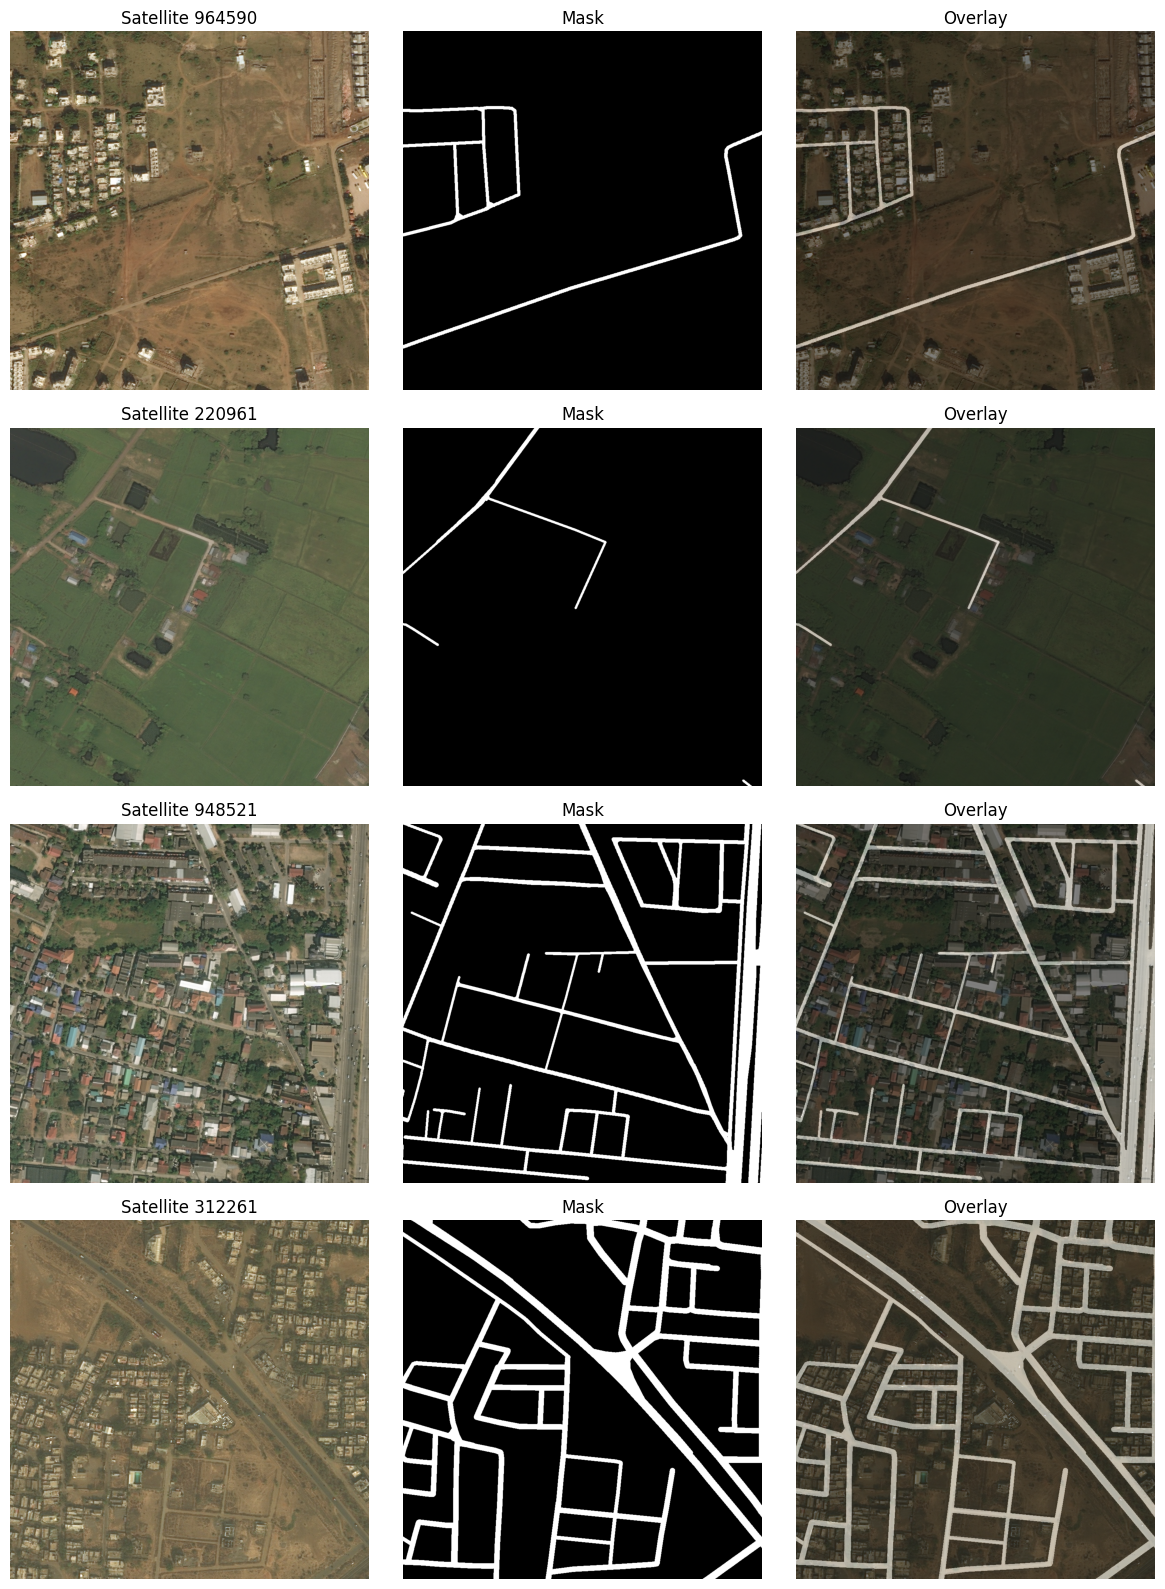
\includegraphics[width=\columnwidth]{images_example.png}
  \caption{Samples from the DeepGlobe training split, with their binary road masks.
           Road pixels are white.
           Notice the variety of terrain types and the range of road widths --
           from wide urban arteries to thin dirt tracks that nearly vanish.}
  \label{fig:examples}
\end{figure}

Looking at \Cref{fig:examples} for just a few seconds is already instructive.
Three observations emerge directly from the images, and each one will constrain our choice
of method.

\textbf{Class imbalance.}
Road pixels are a small minority of each tile.
From a sample of 50 training images, we measured an average road pixel fraction of 4--8\%.
In practice, this means: a classifier that predicts ``no road'' everywhere
would achieve over 92\% pixel accuracy.
This is why we use IoU as our evaluation metric rather than accuracy; IoU penalises false
negatives and false positives equally and cannot be inflated by predicting the majority class.

\textbf{Spectral heterogeneity.}
Road pixels do not cluster neatly in RGB space.
Asphalt in direct sunlight is bright; the same road under tree canopy is dark;
a packed-earth track in the dry season can be almost white.
This implies that any method relying purely on colour thresholds will face an impossible
trade-off: set the threshold too low and you label every bright field as road;
too high and you miss every road in shadow.
This observation puts a hard ceiling on the classical methods we introduce in
\Cref{sec:baselines} before we run a single experiment.

\textbf{Thin, elongated structures.}
After resizing to $256 \times 256$, many rural roads are 3--5 pixels wide.
A model that discards spatial resolution through aggressive downsampling, and only tries to
recover it at the end, will systematically miss these structures; the information was already
gone.
This is a hard requirement, not a preference.
Any architecture we trust must have a mechanism to \textit{preserve} high-resolution spatial
information, not reconstruct it from scratch.
That requirement points directly to U-Net's skip connections,
as we will see in \Cref{sec:unet}.

% ---------------------
\section{Methodology}
\label{sec:method}

Our analysis is structured as a ladder of increasing complexity.
We introduce the simplest method first, identify where it fails, and let that failure motivate
the next step up.
The ladder has three rungs: RGB thresholding, K-Means clustering, and U-Net.

\subsection{Preprocessing}

All images are resized to $256 \times 256$ and normalised using ImageNet channel statistics
($\mu = [0.485, 0.456, 0.406]$, $\sigma = [0.229, 0.224, 0.225]$).
Masks are scaled to $[0,1]$ and binarised at 0.5; no further normalisation applies to them.

\FloatBarrier
\subsection{Data Augmentation}

With only 803 training images, overfitting is a real risk.
We apply the following augmentations \textit{exclusively at training time}: horizontal and
vertical flips (50\% probability each), random 90/180/270-degree rotations (50\% probability),
and affine transforms including rotation ($\pm 12$°), translation ($\pm 5\%$), and scale jitter
($0.95$--$1.05\times$, 40\% probability).
Every spatial transform applies identically to the image and its mask,
so no labelling inconsistency is introduced.

\begin{figure}[htbp]
  \centering
  \includegraphics[width=\columnwidth]{augmentation_preview/augment_overlay_4_presentation_2x2_948521.png}
  \caption{Examples from the training augmentation pipeline. The same road mask is carried
           through flips, rotations, and small affine perturbations together with the input
           image, increasing geometric variety without corrupting the supervision signal.}
  \label{fig:augmentation}
\end{figure}

\Cref{fig:augmentation} illustrates the rationale behind this choice. For road segmentation,
the label is preserved under these transformations, so augmentation gives the model more
geometric diversity while keeping the image--mask correspondence exact.

\subsection{Baselines}
\label{sec:baselines}

\subsubsection{RGB Thresholding}

The first rung of our ladder: classify a pixel as road if its RGB values satisfy a learned
threshold.
Rather than picking thresholds by hand, we apply the two-sample Kolmogorov--Smirnov (KS)
test \cite{kolmogorov1933ks} to find the value that best separates road and non-road pixel
distributions for each colour channel, using a sample of 50 training images.
We tested five strategies (above-threshold, below-threshold, per-channel range, any-channel
above, and a manual bright-pixel rule at (150,150,150)) and selected the one maximising IoU
on the fixed evaluation samples.

Given the spectral heterogeneity we observed in the EDA, we already expected this to struggle;
the experiments will confirm it.

\subsubsection{K-Means Clustering}

K-Means \cite{lloyd1982kmeans} is the natural next step: instead of a fixed threshold, let
the algorithm discover the colour clusters present in the data.
It partitions pixels into $k$ groups in RGB space without any supervision from the masks;
after clustering, we assign each group the label (road or not) that maximises its overlap
with the training masks.
We swept $k \in \{2, 3, 4, 5, 6\}$ and selected $k=2$ by training IoU.

The same spectral limitation applies here: K-Means still examines each pixel in isolation.
A dark-road pixel and a dark-shadow pixel land in the same cluster.
That said, we include it because it gives us a useful reference point; if a neural network
cannot comfortably beat it, we should question the network.

\subsection{U-Net}
\label{sec:unet}

The third rung is where we bring in spatial context.
U-Net \cite{ronneberger2015unet}, proposed by Olaf Ronneberger, Philipp Fischer, and Thomas
Brox (2015) for biomedical image segmentation, is an encoder--decoder architecture whose
defining feature is the \textit{skip connection}: feature maps from each encoder stage
concatenate directly into the matching decoder stage.
That is precisely what the thin-road observation demanded: high-resolution information does
not disappear during downsampling; the skip connections preserve it on a side channel and
reinject it during upsampling.

Our implementation follows the original paper closely:
\begin{itemize}
  \item \textbf{Encoder}: four \texttt{Down} blocks, each applying $2\times2$ max-pooling
        followed by two $3\times3$ convolutions with BatchNorm and ReLU.
        Channel widths: $64 \to 128 \to 256 \to 512$.
  \item \textbf{Bottleneck}: one \texttt{DoubleConv} block at $1024$ channels.
  \item \textbf{Decoder}: four \texttt{Up} blocks applying a $2\times2$ transposed
        convolution, skip-connection concatenation, and \texttt{DoubleConv}.
        The decoder mirrors the encoder in depth and width.
  \item \textbf{Output}: $1\times1$ convolution to a single-channel logit map.
\end{itemize}
The model has 31.0\,M parameters.
We trained it for 30 epochs using the Adam optimiser ($\eta = 10^{-4}$) with
\texttt{ReduceLROnPlateau} (patience\,=\,3, factor\,=\,0.5), binary cross-entropy loss,
and batch size 8 for the initial $256\times256$ resolution experiments.
Training ran on an NVIDIA A10G GPU (24\,GB VRAM) via Modal cloud computing,
completing in roughly 30 minutes. A secondary experiment at $512\times512$ resolution was conducted with batch size 4 due to VRAM constraints, finishing in approximately 2 hours.

% Section on a large pretrained model intentionally removed from the report per project decision.
% U-Net architecture diagram and explanation
\begin{figure}[htbp]
  \centering
  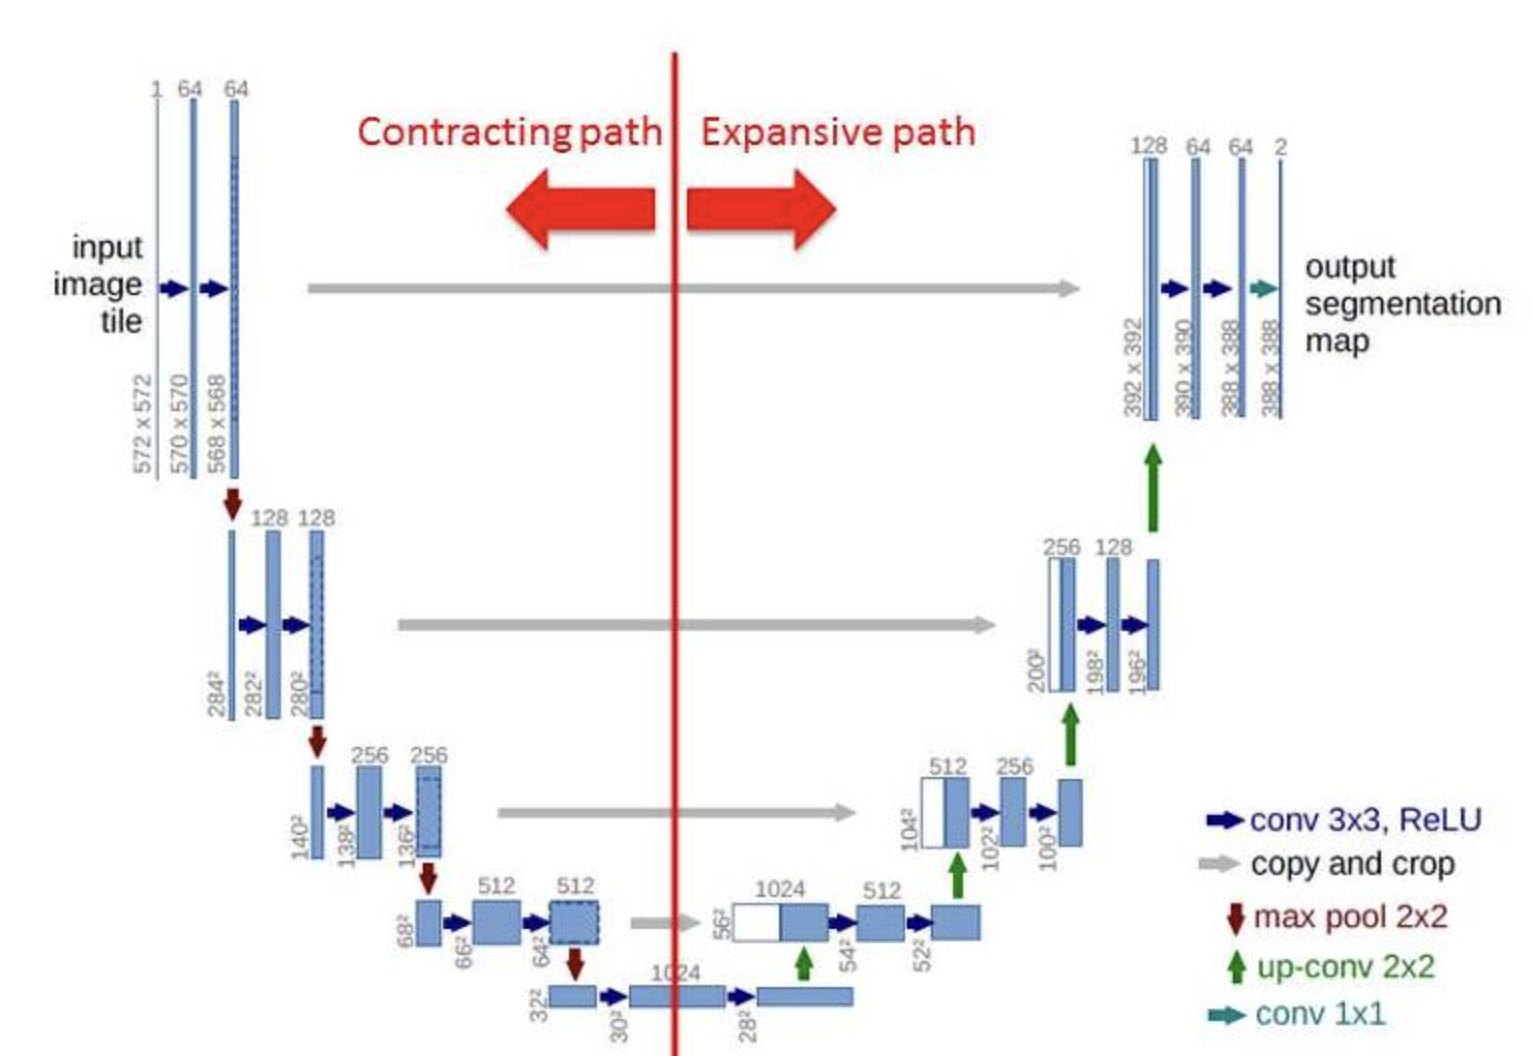
\includegraphics[width=\columnwidth]{../../docs/images/UNetArchitecture.png}
  \caption{Schematic of the U-Net architecture used in this work. Skip
           connections preserve high-resolution features that are critical to
           recovering thin road structures.}
  \label{fig:unet_arch}
\end{figure}

The U-Net diagram in \Cref{fig:unet_arch} summarises the model used in this project.
Its encoder progressively reduces spatial resolution while increasing feature depth,
capturing semantic context; the decoder correspondingly upsamples and fuses encoder
features via skip connections, restoring spatial detail. This design mitigates the
loss of thin linear structures (roads) during downsampling: the skip connections carry
edge and localisation cues from shallow layers directly to the corresponding reconstruction
stages, enabling precise boundary recovery even when global context is necessary for
disambiguation (e.g., differentiating shadows from roads).

In the context of our dataset, the U-Net's advantage is twofold: (1) locality-preserving
reconstruction for thin road edges and (2) an effective trade-off between model size and
representational capacity, allowing training from scratch on limited labelled data.

\FloatBarrier

\subsection{Evaluation Metric}

We report Intersection over Union (IoU), the Jaccard index:
\begin{figure}[htbp]
  \centering
  \begin{minipage}{0.4\linewidth}
    \centering
    \begin{equation}
      \text{IoU} = \frac{|\hat{Y} \cap Y|}{|\hat{Y} \cup Y|}
      \label{eq:iou}
    \end{equation}
  \end{minipage}
  \begin{minipage}{0.4\linewidth}
    \centering
    
\includegraphics[width=0.6\linewidth]{../../assets/iou_diagram.pdf}
  \end{minipage}
\end{figure}
\FloatBarrier

where $Y$ is the ground-truth mask and $\hat{Y}$ the predicted mask.
IoU is symmetric in false positives and false negatives and cannot be inflated by the
background class, which is why we chose it given the class imbalance noted
in~\Cref{sec:eda}.

% ---------------------

\pagebreak
\section{Results}
\label{sec:results}

\subsection{Quantitative Comparison}

\begin{table}[htbp]
  \centering
  \caption{Validation IoU for all methods. For the deep learning models,
           the binarisation threshold was chosen by sweeping $[0.35, 0.50]$
           in steps of 0.05 on the validation set.}
  \label{tab:results}
  \begin{tabular}{lcc}
    \toprule
    Method                  & Val.\ IoU         & Parameters \\
    \midrule
    RGB Thresholding (KS)   & $\sim$0.15--0.25  & -- \\
    K-Means ($k=2$)         & $\sim$0.20--0.30  & -- \\
    U-Net ($512\times512$)  & 0.565             & 31.0\,M \\
    \textbf{U-Net ($256\times256$)} & \textbf{0.588}    & 31.0\,M \\
    \bottomrule
  \end{tabular}
\end{table}
\FloatBarrier

\Cref{tab:results} summarises the main results.
U-Net outperforms the classical baselines by more than 0.30 IoU points.
We discuss possible reasons for this ordering in \Cref{sec:discussion}.
K-Means can isolate some road-coloured pixels, but it fragments easily and
confuses roads with spectrally similar background regions.

Additionally, we observe an interesting dynamic regarding image resolution. 
While downsampling original $1024\times1024$ images to $256\times256$ yielded an IoU of 0.588, increasing the input resolution to $512\times512$ paradoxically slightly lowered the IoU to 0.565. 
This occurs because downsampling heavily blurs thin roads into wider, more prominent patches, making them easier for the model to detect and producing "artificially" higher overlap in low-resolution space. Conversely, at $512\times512$, the roads remain thinner and sharper, but the metric penalises the model more severely for slight pixel misalignments at the boundaries. The higher resolution model preserves the true topology of the road network better, even if the strict exact-pixel matching of IoU does not fully reflect this qualitative improvement.

\textbf{Threshold calibration.}
U-Net outputs raw logits, so we swept the binarisation threshold on the validation set to
find the optimal operating point.

\Cref{fig:curves} shows the U-Net learning curves.
\begin{figure}[H]
  \centering
  \includegraphics[width=\columnwidth]{unet/training_curves.png}
  \caption{Training and validation loss curves for U-Net.}
  \label{fig:curves}
\end{figure}

Qualitatively, U-Net recovers thin rural roads and complex urban intersections with sharp
and connected outlines; these visualisations support the quantitative improvements in
\Cref{tab:results}.
We note that the loss plateaus fairly early; the \texttt{ReduceLROnPlateau} scheduler
triggers a few times (visible as the inflection points) and each trigger produces a small
but consistent improvement.
Together, this tells us that 30 epochs with the chosen augmentation pipeline is a sensible
training recipe for this dataset size, as the model converges cleanly without overfitting.

\subsection{Qualitative Predictions}

\begin{figure}[H]
  \centering
  \includegraphics[width=\columnwidth]{../outputs/unet/unet_prediction_4_valid.png}
  \caption{U-Net predictions on validation images (image, ground-truth,
           prediction, overlay).
           U-Net recovers thin rural roads and complex urban intersections
           with sharp, coherent outlines.}
  \label{fig:unet_preds}
\end{figure}

% Visuals and explicit comparison to a specific large pretrained model removed from the report.
Qualitatively, the U-Net predictions illustrate the model's ability to recover thin and
connected road outlines, supporting the quantitative improvements reported in \Cref{tab:results}.

% ---------------------
\section{Discussion}
\label{sec:discussion}

\textbf{Why classical baselines fail.}
The EDA in \Cref{sec:eda} already gave us the answer before we ran a single experiment.
Both RGB thresholding and K-Means treat every pixel independently, with no knowledge of its
neighbours.
A pixel from a shaded road segment is spectrally identical to a pixel from a forest floor;
the only difference is context, as it sits surrounded by other road-like pixels forming a
long, narrow strip.
Any method that ignores spatial relationships cannot exploit that context; the ceiling on
their performance is set by how spectrally separable road pixels happen to be, and on this
dataset, that answer is: not very.

\textbf{Why U-Net outperforms larger pretrained models.}
This is the more interesting result, and we think it deserves a careful interpretation rather
than a quick dismissal.
Larger pretrained models often aggregate multi-scale context and benefit from ImageNet
backbones. However, the task here is dominated by thin, local structures where what matters
is not global context but the preservation of high-resolution spatial detail.
U-Net's skip connections preserve that detail directly and therefore align better with the
task's inductive bias. ImageNet pretraining may also be less helpful for satellite imagery,
which differs substantially from natural photographs.

\textbf{Paths forward.}
Several directions could push performance further from where we are now.
First, replacing binary cross-entropy with a combined BCE+Dice loss would directly optimise
a proxy of IoU and helps under class imbalance \cite{milletari2016vnet}.
Second, we experimented with training at $512 \times 512$ rather than $256 \times 256$ to reduce spatial
aliasing. While it helped preserve thinner structures visually, it dropped the IoU marginally due to the strictness of high-resolution pixel-perfect matching. Exploring boundary-aware loss functions could help align the qualitative improvement with the quantitative metric.
Third, test-time augmentation (averaging predictions over flipped and rotated versions of
each test image at no extra training cost) typically yields 1--3 IoU points in segmentation
tasks.
We could also consider using U-Net predictions as a spatial prior for a context head of a
larger model, though that would step outside the scope of this coursework.

\textbf{Limitations.}
Our evaluation covers only the DeepGlobe validation set, which shares the same geographic
distribution (South and Southeast Asia) as the training data.
We have no evidence that the model generalises to different regions, sensors, or seasons.
The test-set IoU could not be evaluated since the ground truth labels are not publicly available.
Finally, the $256 \times 256$ resizing is a known bottleneck; it discards spatial detail
that likely matters for the smallest road categories.

% ---------------------
\section{Conclusion}
\label{sec:conclusion}

We framed road segmentation as binary semantic segmentation and compared methods of
increasing complexity on the DeepGlobe dataset.
The performance ordering closely mirrors each method's ability to exploit spatial context:
classical pixel-level baselines (IoU $\leq 0.30$) fall below the deep-learning approaches we
report, and U-Net (IoU 0.588) outperforms the alternatives because its skip-connection
architecture directly addresses the thin-road requirement we identified in the exploratory
analysis, even before a single epoch of training.

The lesson we take from this work goes beyond road segmentation.
A careful reading of the data is more valuable than a reflexive choice of the most powerful
model available.
Understanding that roads are thin, sparse, and spectrally heterogeneous pointed us to
U-Net's design from the beginning; the results confirmed that intuition.
For future improvements, exploring the combined loss strategies and higher-resolution
training pipelines identified in the discussion would be the most promising next steps.

% ---------------------
\bibliographystyle{IEEEtran}
\bibliography{report}

\end{document}
